\documentclass[lecture.tex]{subfiles}

\begin{document}

%\section{TP n$^{\circ}$2 : Matériaux - Traction }
\subsubsection{Objectifs du TP}
Les objectifs de ce TP sont de :
\begin{itemize}[label=\ding{110},font=\tiny]
\item Déterminer le module d'Young à partir du diagramme d'essai de traction pour différents matériaux ;
\item Acquérir un sens physique de l'élasticité des matériaux ;
\item Savoir prendre en compte des précautions nécessaires à l'élimination des phénomènes parasites nuisant aux observations des caractéristiques mécaniques ;
\item \'Etudier un diagramme d'essai de traction complet.
\end{itemize}

\subsubsection{Manipulations}
Dans un premier temps,  pour différents matériaux, vous allez déterminer le module d'Young $E$ qui est une propriété mécanique du matériau caractérisant son élasticité longitudinale. Pour ce faire, vous allez réaliser des essais de traction permettant un relevé sous différentes charges du déplacement relatif des deux têtes de serrage des éprouvettes. À partir de ces mesures, vous allez pouvoir tracer le diagramme contrainte / allongement relatif, en vue d'accéder au module d'Young,
%Il s'agit donc pour vous dans un premier temps de déterminer ce module d'Young à partir de la pente charge / déplacement ou contrainte / déformation sans sortir de la zone élastique (PVC : $500\,N$ et alliages : $1000\,N$ au maximum).\\

Dans un second temps (voir section~\ref{Sec_DiagEssai}), vous aurez à déterminer la valeur précise de la limite d'élasticité des matériaux et à aller jusqu'à la rupture (pour les éprouvettes fournies spécialement).

\paragraph*{Description du matériel}
\noindent

%\begin{minipage}{\textwidth}
  %
  %\begin{minipage}[l]{0.6\textwidth}
    Pour réaliser les expériences, on dispose de :
    \begin{itemize}[label = \ding{110}, font = \tiny]
      \item Un cadre triangulaire (voir Fig.~\ref{Fig_banc} avec chapes supérieure et inférieure permettant de placer l'éprouvette avec poutre dynamométrique, vis de charge, volant de manœuvre et équipé d'un comparateur réglé ;
      \item Deux piges en laiton ;
      \item Une pige à tête PVC ;
      \item Deux comparateurs équipés de touches orientables montées sur rallonge ;
      \item Plusieurs éprouvettes de traction de différentes tailles et de différents matériaux (aluminium, acier, PVC).
    \end{itemize}
  %\end{minipage}
  %\begin{minipage}{0.38\textwidth}
    \begin{figure}[h!]
      \centering
      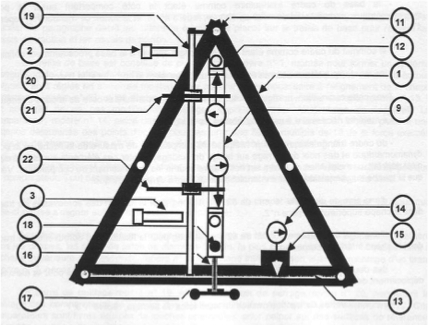
\includegraphics[scale=0.8]{Fig_banc.png}
      \caption{Configuration du banc pour l'essai de traction.}
      \label{Fig_banc}
    \end{figure}
  %\end{minipage}
%\end{minipage}

\medskip
%\vspace{\baselineskip}

Les éprouvettes destinées à la détermination du module d'Young ont une longueur entre têtes de $370\, mm$ et celles destinées à la rupture ont une longueur entre têtes de $50\, mm$.

\paragraph*{Préliminaires à l'expérience d'élasticité}

\begin{description}
  \item[$\bullet$] Dans l'exécution des essais de traction, la force $\vec{F}$ doit s'exercer selon l'axe de l'éprouvette (voir Fig.~\ref{Fig_Eprouvette}). Toute flexion de celle-ci se trouve alors éliminée. Dans ces conditions, on peut admettre que toutes les fibres longitudinales subissent le même allongement et que les sections transversales qui sont initialement planes et perpendiculaires à l'axe de l'éprouvette continuent à l'être après traction.
\begin{figure}[h!]
\begin{center}
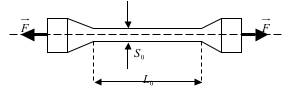
\includegraphics[scale=0.8]{Fig_Schema.png}
\caption{Représentation schématique d'une éprouvette et notations utilisées.}
\label{Fig_Eprouvette}
\end{center}
\end{figure}

%Les valeurs des raideurs d'éprouvette mesurées avec les comparateurs du banc sont suffisamment précises pour déterminer l'influence de chaque paramètre intervenant dans le comportement des structures en traction. C'est le but principal des expériences illustrant les notions fondamentales des traités de résistance des matériaux de tous niveaux.

\item[$\bullet$] \textbf{Procédure pour la mise en place du banc de traction}
\begin{enumerate}[label = \alph*)]
\item Placez une des têtes de la première éprouvette à étudier dans la chape supérieure (repère $n^{\circ}12$) et introduisez la pige de diamètre $10\, mm$ et de $62\, mm$ de long (repère $n^{\circ}2$) pour lier l'éprouvette à cette chape, tout en soutenant l'autre tête avec la main pour éviter de plier plastiquement les tôles minces ;
\item Placez la seconde tête dans la chape inférieure $n^{\circ}18$ et tournez le volant de manœuvre afin d'introduire la pige de diamètre 10 mm et de 82 mm de long, repère $n^{\circ}3$ dans les alésages de la chape et de cette tête ;
\item Alignez l'éprouvette et les chapes en tournant le volant dans le sens horaire jusqu'à une légère déviation ($1$ à $\frac{2}{100} mm$) de l'aiguille du comparateur de mesure du déplacement de la poutre dynamométrique (repère $n^{\circ}14$). Ce comparateur permettra de lire la valeur de l'effort de traction ;
\item Montez les comparateurs de mesure des déplacements des éprouvettes (repères $n^{\circ}21$ et $n^{\circ}22$) sur la tige de guidage (repère $n^{\circ}19$) en introduisant leur rallonge dans les noix de serrage (repère $n^{\circ}20$). La petite rallonge doit être montée vers le sommet du triangle noir ;
\item Veillez à visser l'extrémité des palpeurs des comparateurs au début du TP et à chaque changement d'éprouvette ;
\item Réglez la position des comparateurs, touche orientable perpendiculaire à l'axe de déplacement en contact avec les faces des têtes des éprouvettes ; l'axe de translation des comparateurs doit être parallèle à l'axe de l'éprouvette essayée ;
\item Faites un premier zéro de tous les cadrans des comparateurs. Le banc est prêt pour un essai de traction.
\end{enumerate}
\vspace{\baselineskip}

Remarque : pour changer d'éprouvette après avoir ramené la charge à zéro, il suffit de dégager les comparateurs de mesure de déplacements des extrémités de l'éprouvette en desserrant les noix et en les faisant pivoter autour de la tige de guidage avant de remplacer l'éprouvette étudiée par une nouvelle. Remettre ensuite en place les comparateurs de façon à ce que les touches orientables soient en contact avec les têtes de la nouvelle éprouvette et \textbf{après avoir vissé l'extrémité des palpeurs}.

\end{description}

\paragraph*{Conduite opératoire et précautions à prendre}
\label{Sec_JeuInitiaux}

\begin{description}
  \item[$\bullet$] \textbf{Affranchissement des jeux initiaux.}
Pour s'affranchir des problèmes de jeux initiaux du montage, il suffit de mettre une légère pré-charge de quelques dizaines de Newton avant de faire un zéro de tous les comparateurs.
Après ce calage de l'éprouvette dans ces attaches et avant d'effectuer une série de mesures, il vous est conseillé de faire une première mise en charge progressive en restant dans le domaine élastique. Ceci permet alors de vérifier que les comparateurs dévient bien et sont donc en contact avec les têtes de serrage sur toute l'étendue de la mesure prévue. Après une première décharge, une légère correction des zéros des comparateurs peut être nécessaire. Cette procédure d'initialisation garantit une bonne répétitivité des mesures. À noter qu'il faut que les comparateurs reviennent à zéro après une charge et une décharge afin de stabiliser le montage.

  \item[$\bullet$] \textbf{Limites de charges.}
Pour les éprouvettes en PVC, vous ne dépasserez pas $500\, N$ de charge (c'est-à-dire un demi-tour de cadran du comparateur). Pour les éprouvettes en alliages et en aluminium, vous pourrez aller jusqu'à $1000\, N$ (un tour de cadran).

\item[$\bullet$] \textbf{Procédure et recommandations.} L'expérience consiste à contraindre par palier l'éprouvette en augmentant par incrément de $10\, daN$, par exemple, la charge en tournant le volant de manœuvre toujours dans le sens horaire pour éviter les phénomènes de jeux. Il est recommandé :

\begin{itemize}[label =\ding{110}, font = \tiny]
%\item D'arriver au point de mesure en tournant le volant toujours dans le sens horaire pour éviter les phénomènes de jeux ;
\item De prendre les mesures de l'épaisseur et de la largeur des éprouvettes précisément à l'aide d'un pied à coulisse.
\item De tapoter légèrement avec les doigts les montants du cadre triangulaire avant de relever les valeurs effectivement atteintes par les comparateurs de mesure des déplacements des éprouvettes. Ceci doit être fait pour s'affranchir des frottements résiduels et autres phénomènes d'hystérésis mineurs pouvant entacher la mesure de la flèche de l'éprouvette qui est cruciale pour la détermination des caractéristiques mécaniques recherchées ;
\end{itemize}
\vspace{\baselineskip}
Remarque : l'attention à accorder à la mesure du déplacement relatif des deux têtes des comparateurs reste primordiale pour la qualité des résultats.

\vspace{\baselineskip}

\item[$\bullet$] \textbf{Pourquoi l'utilisation de deux  comparateurs ?}
Le faible niveau des valeurs des déplacements impose l'emploi de deux comparateurs. En effet, les quelques centièmes de millimètres de déplacement de la tête de serrage supérieure de l'éprouvette pourraient conduire à des erreurs très grandes. Le montage n'a pas une rigidité infinie bien qu'elle soit supérieure à celle des éprouvettes et il faut extraire sa déformée par\textbf{ une mesure différentielle} pour n'observer que le déplacement de l'éprouvette.
Considérer en effet que la tête de serrage supérieure reste immobile pendant la charge serait une hypothèse conduisant à des erreurs trop importantes pour accorder une signification aux caractéristiques mécaniques relevées de cette manière.

\end{description}

\subsubsection{Questionnaire}
\paragraph*{Étude du domaine élastique}
\begin{enumerate}
\item \ding{46} Quelle relation relie la charge $F$ (force de traction),  l'allongement relatif $\varepsilon_r$  lié à la longueur de l'éprouvette, le module d'Young $E$ et l'aire $S$ de la section de l'éprouvette ? Donner le nom de cette loi.
\item Tracez la contrainte $\sigma$ en fonction de l'allongement relatif $\varepsilon_r$. Faîtes deux séries de mesures sur une des quatre éprouvettes. Pensez à la procédure d'affranchissement des jeux initiaux présentée Sec.~\ref{Sec_JeuInitiaux}.
\item Déterminez le module d'élasticité longitudinale $E$ des matériaux testés en calculant la moyenne des deux modules d'Young $E$ qui ont été trouvés lors des essais.
\item Comparer vos résultats expérimentaux du module d'Young avec les résultats obtenus par extensométrie fournies Table.~\ref{Fig_Ext}.
\item Calculez par la méthode de propagation des incertitudes, l'incertitude sur vos valeurs expérimentales du module d'Young $E$ à partir de l'évaluation des incertitudes sur les mesurandes directs.
%\item Comment expérimentalement mettre en évidence la proportionnalité entre l'allongement et la charge ? entre l'allongement et l'inverse de la section ? entre l'allongement et l'inverse de E ?
%\item Peut-on en déduire que la déformation des matériaux dans le domaine élastique est proportionnelle à la contrainte appliquée et inversement proportionnelle au module d'élasticité longitudinale du matériau ?
%\item Les matériaux testés sont-ils élastiques ?
%\item Au-delà de leur limite d'élasticité, sont-ils élastiques ?
\end{enumerate}

\begin{table}[h!]
\caption{Module d'élasticité longitudinale obtenu par extensométrie.}
\begin{center}
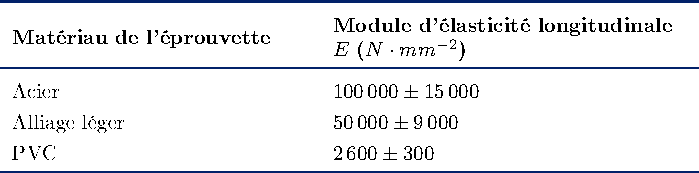
\includegraphics[scale=1]{Table_Extensometrie.pdf}
\label{Fig_Ext}
\end{center}
\end{table}


\paragraph*{Etude du diagramme d'essai de traction complet}\par
\label{Sec_DiagEssai}
Dans cette expérience, vues les faibles épaisseur et largeur de l'éprouvette, il faut prendre des pas d'efforts les plus petits possibles tant qu'on n'a pas dépassé la contrainte limite élastique. Ensuite, vous pouvez augmenter le pas d'effort.

\begin{enumerate}[resume]
\item Tracez le diagramme d'essais de traction complet.
\item Relevez la charge limite à la rupture pour chaque matériau.
\item Relevez l'allongement total de l'éprouvette à la rupture.
\item \ding{46} Qu'est ce que la striction ? Caractérisez l'instant d'apparition de la striction.
\item En vous intéressant au domaine élastique uniquement, déterminez la loi d'élasticité. Explicitez le module d'Young du matériau étudié.
\item Quantifiez la contrainte $\sigma_{0,2}$ à $0.2\,\%$ du matériau étudié.
\item En vous intéressant au domaine plastique, écrivez la loi de plasticité complète à partir du diagramme d'essai de traction obtenu. On rappelle que dans ce domaine on peut écrire que $\sigma = k\epsilon^n$, où $n$ désigne  le coefficient d'écrouissage et $k$ un coefficient de proportionnalité.
\end{enumerate}

%\subsubsection{Loi de plasticité}
%A partir de la courbe obtenue sur l'aluminium et en vous intéressant au domaine élastique et au domaine plastique :
%\begin{enumerate}[resume]
%\item Modélisez cette courbe dans le domaine élastique (on fera l'hypothèse de linéarité dans ce domaine).
%\item \`{A} partir de cette courbe, et en vous intéressant au domaine plastique, tout en sachant que dans ce domaine on peut écrire que $\sigma = k\epsilon^n$ (avec $n$ qui est le coefficient d'écrouissage et $k$ qui est un coefficient de proportionnalité), écrivez la loi de plasticité complète à partir des résultats expérimentaux.
%\end{enumerate}
%Pour répondre à cette partie, on pourra passer en représentation logarithmique.
%

%\subsubsection{Hors TP : Thèmes théoriques de réflexion, à revoir dans les cours, TD, livres, internet..etc}
%\begin{itemize}[label =\ding{110}, font =\tiny ]
%\item Coefficient d'écrouissage ;
%\item Quantification de $\sigma_{0,2}$ pour un matériau ;
%\item Loi de plasticité. Dans le domaine de la plasticité on peut écrire que $\sigma = k\epsilon^n$ (avec $n$ qui est le coefficient d'écrouissage et $k$ qui est un coefficient de proportionnalité) ;
%\item Proportionnalité entre l'allongement et la charge, entre l'allongement et l'inverse de la section, entre l'allongement et l'inverse de $E$.
%\end{itemize}


\end{document}
